%+210 to left and -210 to right if I want to move one subfigure.

\begin{figure}[!h]
%\vspace{-1pt} %takes away some white space before figure
\centering
\iftrue
\begin{subfigure}[b]{1.0\textwidth}
\centering
	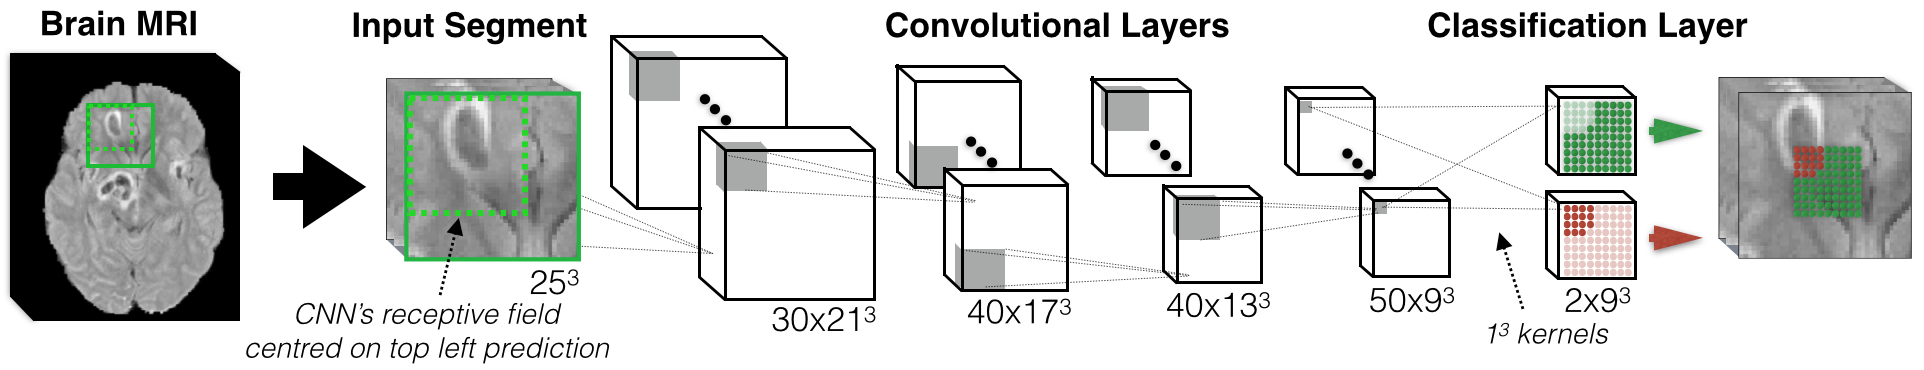
\includegraphics[clip=true, trim=0pt 0pt 0pt 0pt, width=1.0\textwidth]{figures/methodSection/cnnSystem/baselineDense.png}
\end{subfigure}
\fi
\caption{Our baseline CNN consists of four layers with $5^3$ kernels for feature extraction, leading to a receptive field of size $17^3$. The classification layer is implemented as convolutional with $1^3$ kernels, which enables efficient \textit{dense-inference}. When the network segments an input it predicts multiple voxels simultaneously, one for each shift of its receptive field over the input. Number of FMs and their size depicted as (\textit{Number $\times$ Size}).}
\label{fig:cnnBaseline}
\end{figure}
